\hypertarget{v6-ux5173ux952eux6d88ux878dux4e0eux5f00ux53d1ux7ed3ux679c}{%
\section{V6 关键消融与开发结果}\label{v6-ux5173ux952eux6d88ux878dux4e0eux5f00ux53d1ux7ed3ux679c}}

\hypertarget{ux540cux4e00-100-episode-ux5f00ux53d1-bank}{%
\subsection{同一 100-episode 开发 bank}\label{ux540cux4e00-100-episode-ux5f00ux53d1-bank}}

V6 的 E0、E-Oracle、E1、E2 和 D1 全部使用同一组 100 个开发 episode，因此可以做直接的描述性比较：

\begin{longtable}[]{@{}lrrrr@{}}
\toprule\noalign{}
模型 & Benchmark & Strict & Exit/Entry & 20-step hold \\
\midrule\noalign{}
\endhead
\bottomrule\noalign{}
\endlastfoot
E0 Vision & 62\% & 34\% & 59.68\% & 53\% \\
E-Oracle & 75\% & 42\% & 53.33\% & 65\% \\
E1 & 65\% & 22\% & 73.85\% & 54\% \\
E2 & 78\% & 38\% & 62.82\% & 56\% \\
D1 & 66\% & 31\% & 57.58\% & 53\% \\
\end{longtable}

\begin{figure}
\centering
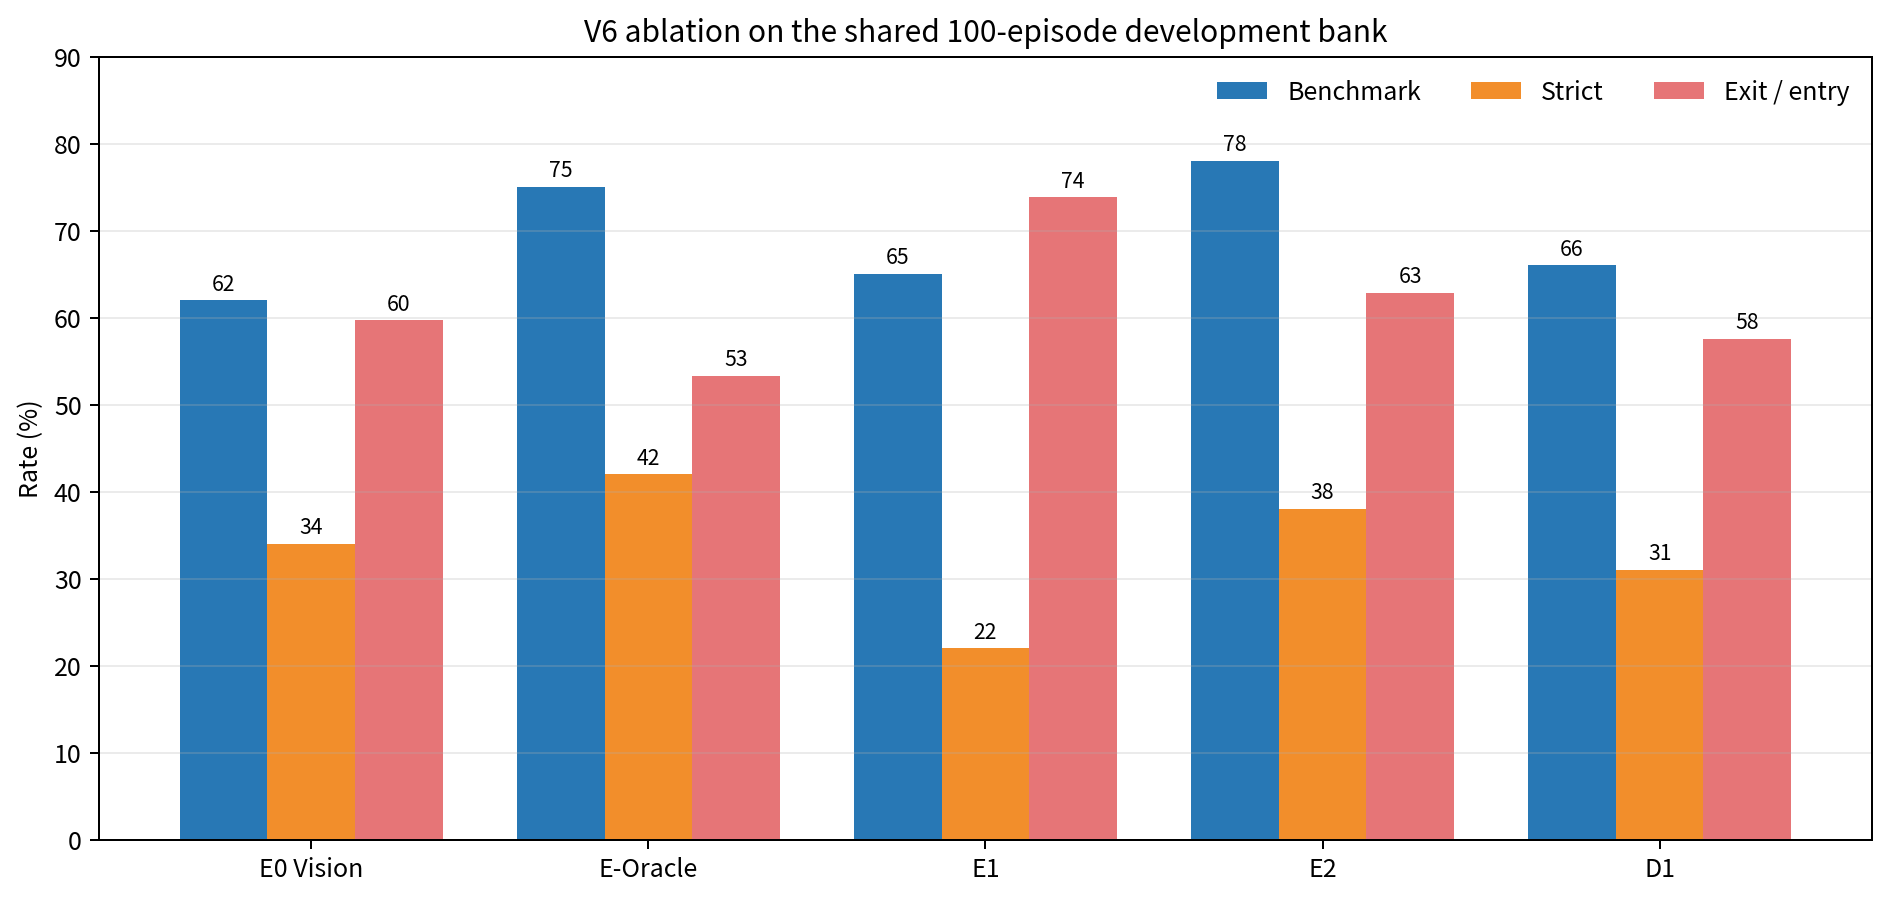
\includegraphics[width=\linewidth]{figures/06_v6_ablation.png}
\caption{V6 同 bank 消融}
\end{figure}

\textbf{图 7｜V6 消融。} 五个策略共享旧 100-episode development bank。Benchmark、Strict 为 episode rate；Exit/Entry 是以各策略自身 entry 为分母的条件比例，不能把较低 exit 单独解释为更强 hold。该图属于开发阶段，不与后面的独立 confirmation 或 frozen test 连成趋势。

E1 的 Benchmark 从 62\% 小幅升到 65\%，但 Strict 从 34\% 降到 22\%，Exit/Entry 恶化到 73.85\%。离线 state/action loss 能够下降，却没有转换成稳定 hold。这说明原 AWAC CNN 学到的主要是满足动作模仿所需的静态特征，冻结它之后，GRU 很难从 latent 中恢复已在 encoder 中被丢掉的姿态细节和速度信息。时序模块不能凭空重建输入表征未保留的动态。

E2 仅允许 estimator 私有 CNN 的最后一个 block 和 projection 适配，Benchmark 达到 78\%，Strict 38\%。与 E1 相比，最后一层视觉适配同时恢复 acquisition 和部分 hold，说明真正关键的组件不是单纯增加 GRU 参数，而是让高层视觉特征对 object/target rotation、angular velocity 和 action-sensitive state 重新可分。它也与 V1 temporal shuffle 几乎不退化的现象呼应：基础 encoder 没有充分保留帧序动态，E2 的稠密监督在靠近输出端的位置对其进行了有目标的修正。

但 E2 在旧开发 bank 上没有通过 V6 当时冻结的 exit guard。其 Exit/Entry 为 62.8205\%，容许上限为 62.6774\%，只高 0.1431 percentage point。按照预先规则，\nolinkurl{STOP_V6_PROMOTION_GATE_NOT_MET} 必须保留，不能因为差距很小或后来结果好就改写成当时已经通过。这个历史 STOP 体现的是开发协议纪律，不等于 E2 方法被永久判定无效。

\hypertarget{d1-ux4e3aux4ec0ux4e48ux4e0dux80fdux66ffux4ee3-e2}{%
\subsection{D1 为什么不能替代 E2}\label{d1-ux4e3aux4ec0ux4e48ux4e0dux80fdux66ffux4ee3-e2}}

D1 从 student policy 新访问的 300 episodes、60,000 transitions 中加入数据，并与历史 state-distillation source 混合再训练。结果为 66\% Benchmark、31\% Strict、57.58\% Exit/Entry。表面看，它的 exit ratio 比 E2 更低，甚至略优于 E0；但 Benchmark 也从 E2 的 78\% 降到 66\%，entry 数减少会机械改变 Exit/Entry 的分母。D1 的 E0 paired benchmark wins/losses/ties 为 27/29/44，没有形成净 acquisition 收益。

这个现象不能简单写成``DAgger 改善了 hold''。更准确的解释是，普通 student-visited aggregation 改变了训练分布，使模型对 student 偏离状态拟合得更多，却损害了 E2 已经形成的目标获取表征。新数据未必提供与原 source 同质量的 teacher coverage，且统一 loss 会让 acquisition 与 hold 竞争。D1 的方向提醒我们：DAgger 不只是``数据越多越好''，关键在于访问分布、标签质量和原能力保护。

\hypertarget{ux5f00ux53d1ux7ed3ux679cux5982ux4f55ux89e6ux53d1ux72ecux7acbux786eux8ba4}{%
\subsection{开发结果如何触发独立确认}\label{ux5f00ux53d1ux7ed3ux679cux5982ux4f55ux89e6ux53d1ux72ecux7acbux786eux8ba4}}

V6.1 没有回到旧 100-episode bank 修改阈值，也没有从 E2 周围再选 checkpoint。它固定原 E2 权重，在全新的 300-episode bank 上同时评估 E0、E2 和 Oracle，并保留逐 episode outcome 用于 paired 统计。这样回答的是不同问题：V6 的结论是``在原开发 gate 下不晋级''，V6.1 的结论是``预先固定的 E2 在独立数据上是否有真实闭环收益''。两者可以同时成立。

这一区分防止两类常见错误。第一，不能因为新 bank 成功就回写旧开发结果，抹掉当时的停止裁决；第二，也不能把旧 bank 的 78\% 当成最终性能，因为它参与过方法选择。最终论证必须以新 confirmation、跨 seed 配方复现和一次性 frozen test 为主。

\textbf{本章结论。} E1 证明``冻结旧视觉特征、只加时序模型''不足，E2 则把有限 last-block adaptation 确定为关键组件。D1 没有恢复 hold，反而损害 acquisition；V6 历史 STOP 保持有效，而 V6.1 对固定 E2 的独立确认是一个新的、不能倒灌到开发流程的证据层级。
